\documentclass[stu, 12pt, letterpaper, donotrepeattitle, floatsintext, natbib]{apa7}
\usepackage[utf8]{inputenc}
\usepackage{comment}
\usepackage{marvosym}
\usepackage{graphicx}
\usepackage{float}
\usepackage{tabularx}
\usepackage[normalem]{ulem}
\usepackage[spanish]{babel} 
\selectlanguage{spanish}
\useunder{\uline}{\ul}{}
\newcommand{\myparagraph}[1]{\paragraph{#1}\mbox{}\\}

% Portada
\thispagestyle{empty}
\title{\Large Aplicativo Web para el Servicio de Comedores de la Universidad Industrial de Santander}
\author{Mauricio Marín - 2215634 \\Miguel Hernández - 2214003 \\Sergio Gómez - 2214106 \\Michael Rueda - 2204131}
\affiliation{Universidad Industrial de Santander}
\course{F1: Ingeniería del Software I}
\professor{Emilio Cárcamo}
\duedate{02 de Octubre de 2024}
\begin{document}
\maketitle


% Índices
\pagenumbering{roman}
    % Contenido
\renewcommand\contentsname{\largeÍndice}
\tableofcontents
\setcounter{tocdepth}{2}
\newpage

% Cuerpo
\pagenumbering{arabic}



\section{Introducción}
El servicio de comedor estudiantil de la Universidad Industrial de Santander es un programa subvencionado de atención a los estudiantes de pregrado presencial de la sede Bucaramanga, que brinda durante los periodos académicos una alimentación nutritiva y balanceada, para contribuir a mejorar su calidad de vida y así evitar su deserción o aumento del tiempo de terminación de su plan de estudios \citep{UIS2024}. Considerando lo anterior, y que otras utilidades como el carnet estudiantil ya cuentan con su contraparte digital \citep{UIS_Carnet_Digital}, surge la necesidad de modernizar y optimizar la gestión de dicho servicio mediante el desarrollo de un aplicativo web, independiente de los demás sistemas institucionales, que permita a los estudiantes consultar los menús diarios, tramitar de forma eficiente excusas por inasistencias y recibir notificaciones importantes, facilitando de esa manera el acceso a la información y mejorando su experiencia como usuarios.

La implementación de esta herramienta busca agilizar los procesos administrativos y fomentar una mayor satisfacción entre los beneficiarios del servicio. De igual forma, su desarrollo responde a la creciente demanda de soluciones digitales que simplifiquen la vida cotidiana de los estudiantes y les brinden un acceso más directo y rápido a los recursos disponibles. Finalmente, se espera que esta solución contribuya a una gestión más efectiva del programa de comedores en términos de usabilidad, permitiendo a los encargados gestionar rápidamente sus operaciones para satisfacer las necesidades de la comunidad universitaria.


\newpage
\section{Identificación de Necesidades} 

\subsection{Mundo del Problema}
El servicio de comedor estudiantil de la Universidad Industrial de Santander en la sede Bucaramanga enfrenta varias problemáticas que afectan la experiencia de los estudiantes. Una de las principales dificultades es el acceso limitado a la información actualizada y completa sobre los menús diarios. Actualmente, la institución utiliza Instagram para mostrar los alimentos correspondientes a la semana, pero esta opción no es accesible para todos los estudiantes debido a que requiere obligatoriamente una cuenta. Además, las publicaciones en dicha red social carecen de información nutricional detallada, lo cual es importante para aquellos estudiantes que necesitan seguir dietas específicas o tengan restricciones alimentarias.

Otra problemática significativa es el proceso de trámite de excusas por inasistencia a alguna comida. Este proceso se realiza a través del sistema de estudiantes de la universidad, pero resulta ser tedioso y poco directo debido a la cantidad de pasos que se deben seguir. La falta de un sistema eficiente y más directo para gestionar las excusas puede generar confusión entre los estudiantes y llevar a sanciones innecesarias o involuntarias. De igual forma, no existe un mecanismo de notificación que informe a los estudiantes si han faltado a alguna comida y que deben tramitar una excusa antes de las próximas 24 horas para evitar sanciones.

\newpage
\subsection{Requerimientos Funcionales}

\begin{figure}[H]
	\caption[]{Primer Requerimiento Funcional}
	\label{Primer Requerimiento Funcional}
	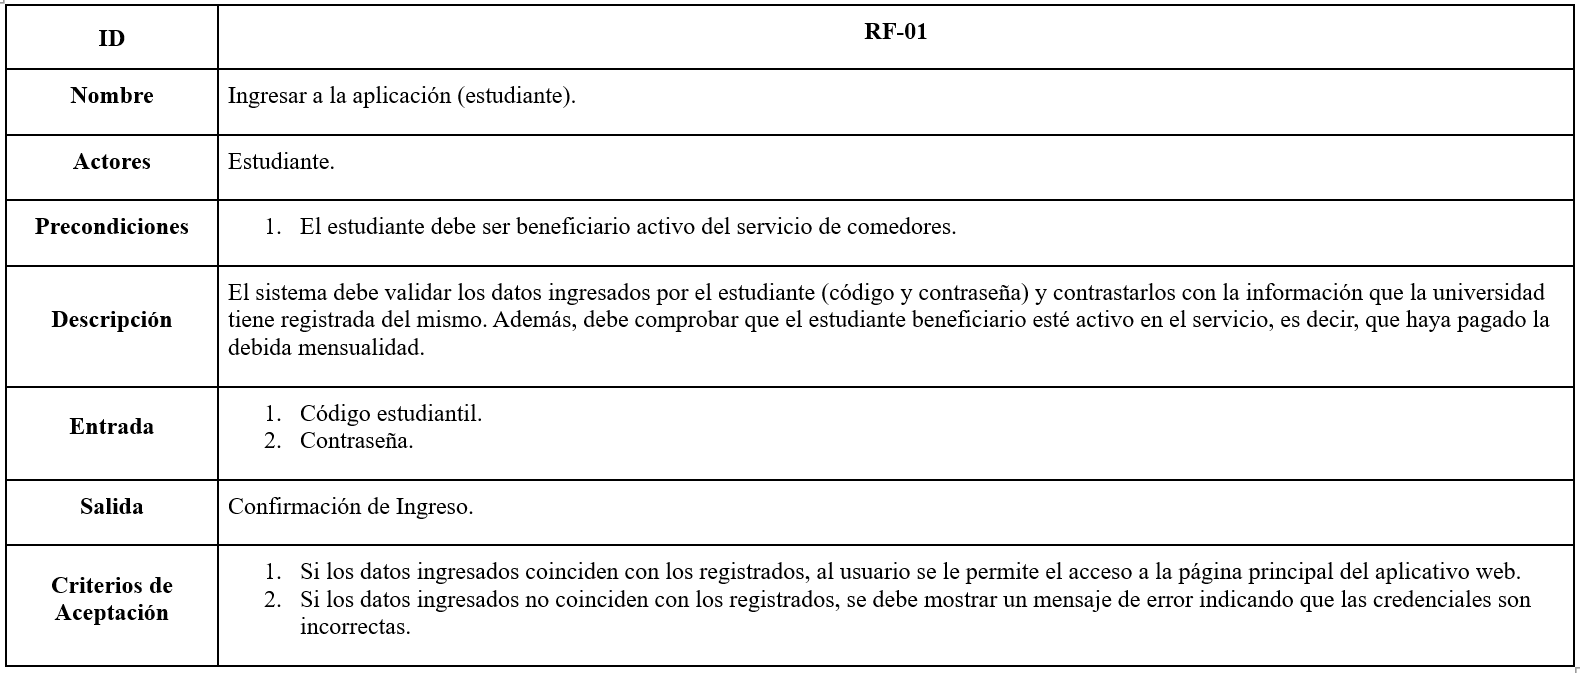
\includegraphics[width=1\linewidth]{Requerimientos Funcionales/1. Requerimiento Funcional.png}
\end{figure}

\begin{figure}[H]
	\caption[]{Segundo Requerimiento Funcional}
	\label{Segundo Requerimiento Funcional}
	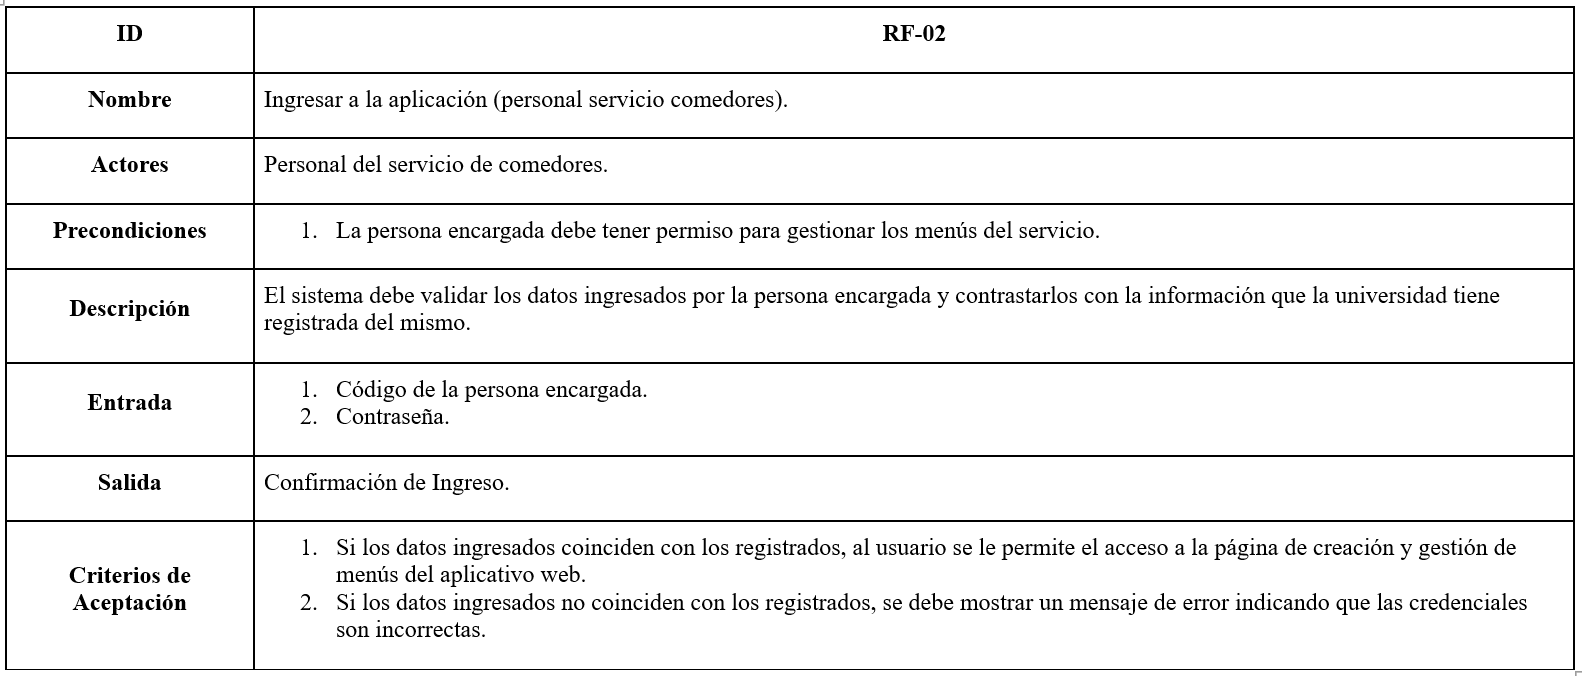
\includegraphics[width=1\linewidth]{Requerimientos Funcionales/2. Requerimiento Funcional.png}
\end{figure}

\begin{figure}[H]
	\caption[]{Tercer Requerimiento Funcional}
	\label{Tercer Requerimiento Funcional}
	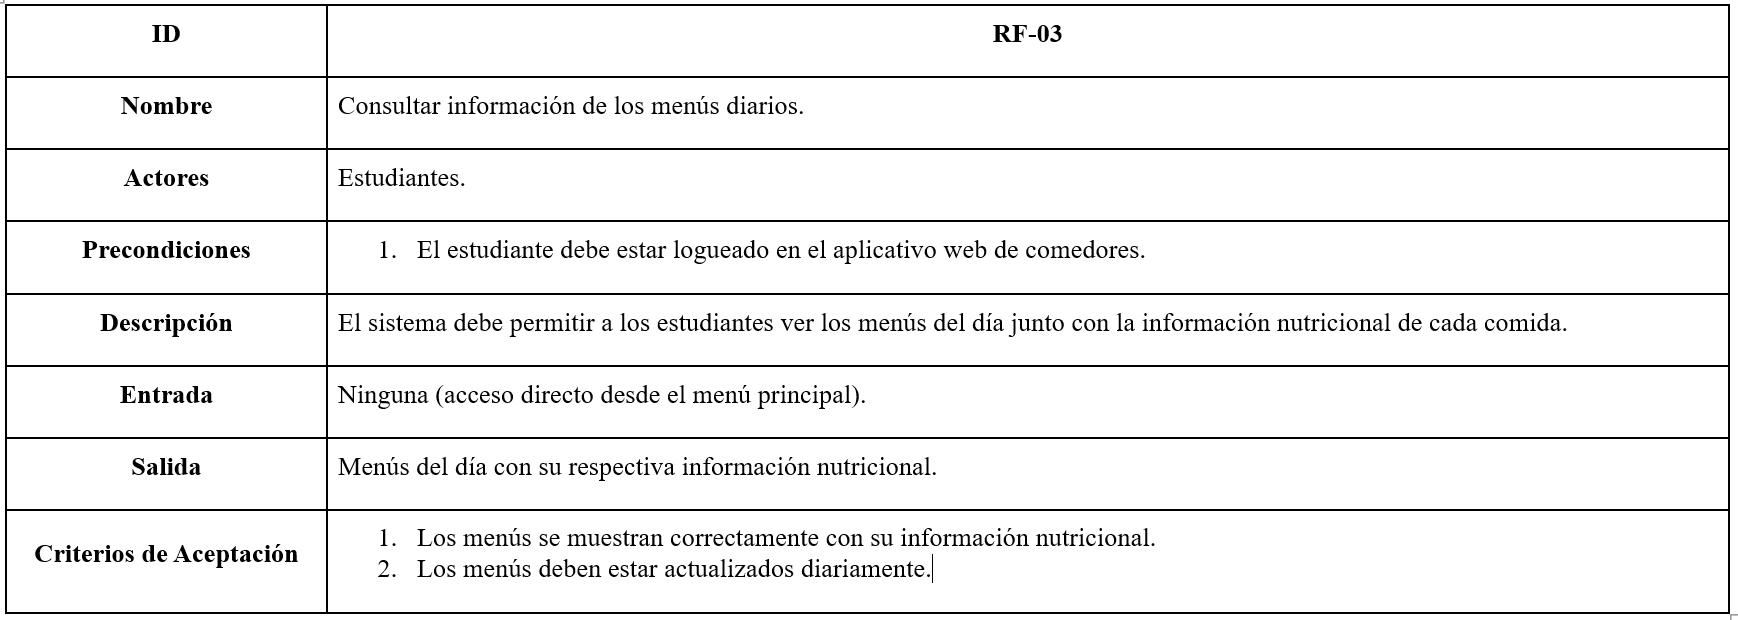
\includegraphics[width=1\linewidth]{Requerimientos Funcionales/3. Requerimiento Funcional.png}
\end{figure}

\begin{figure}[H]
	\caption[]{Cuarto Requerimiento Funcional}
	\label{Cuarto Requerimiento Funcional}
	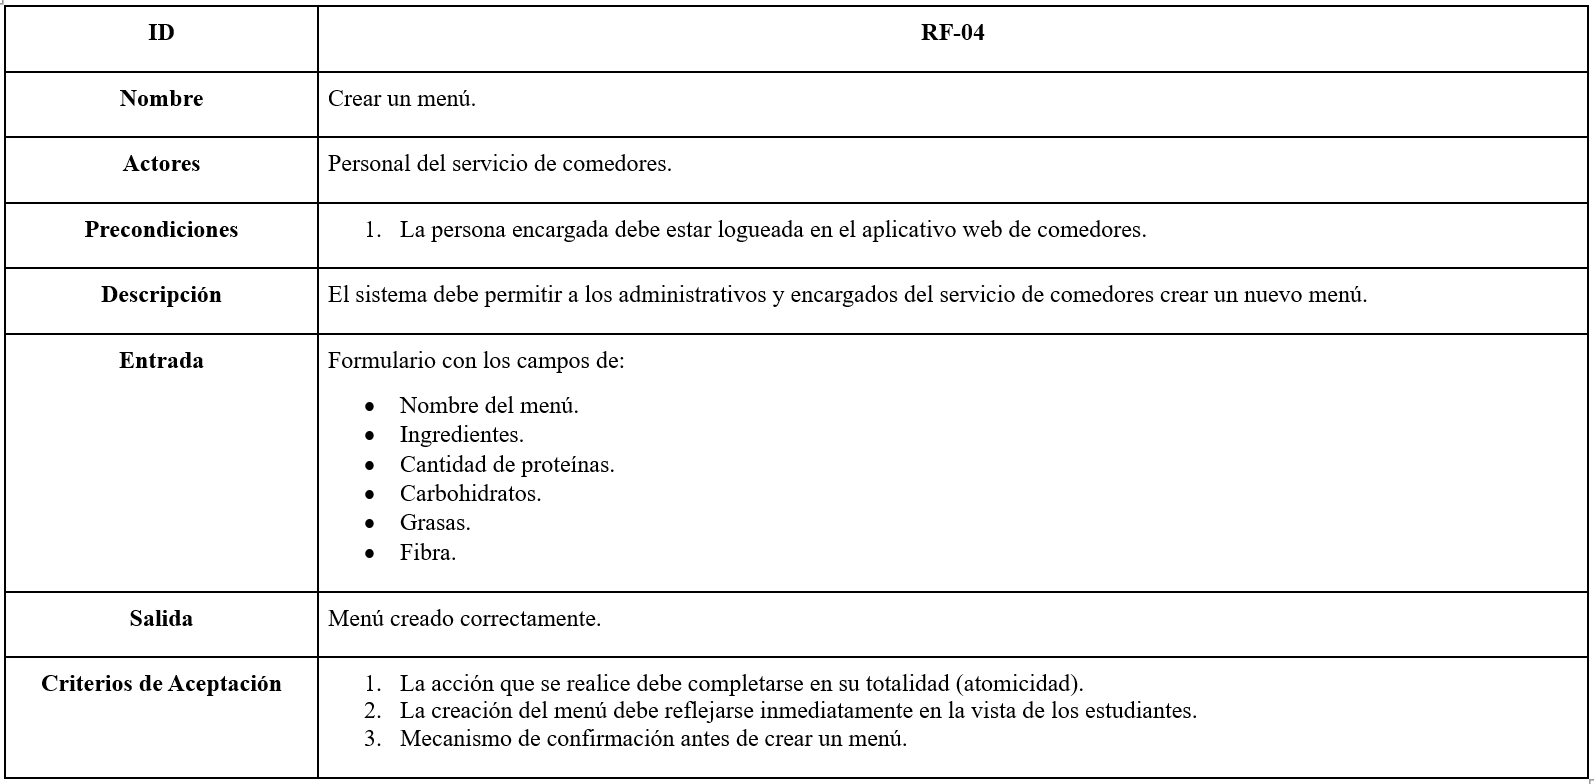
\includegraphics[width=1\linewidth]{Requerimientos Funcionales/4. Requerimiento Funcional.png}
\end{figure}

\begin{figure}[H]
	\caption[]{Quinto Requerimiento Funcional}
	\label{Quinto Requerimiento Funcional}
	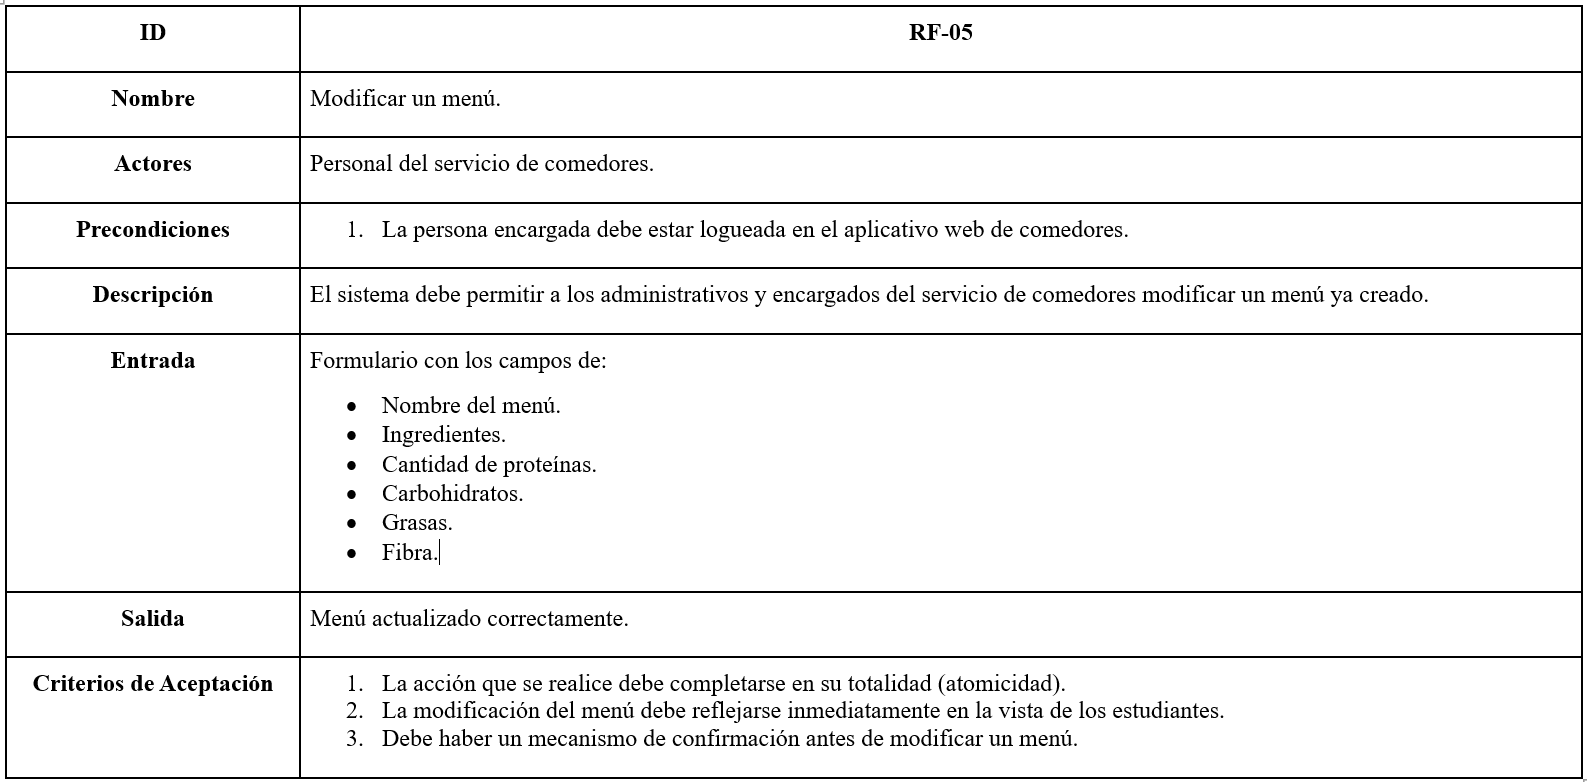
\includegraphics[width=1\linewidth]{Requerimientos Funcionales/5. Requerimiento Funcional.png}
\end{figure}

\begin{figure}[H]
	\caption[]{Sexto Requerimiento Funcional}
	\label{Sexto Requerimiento Funcional}
	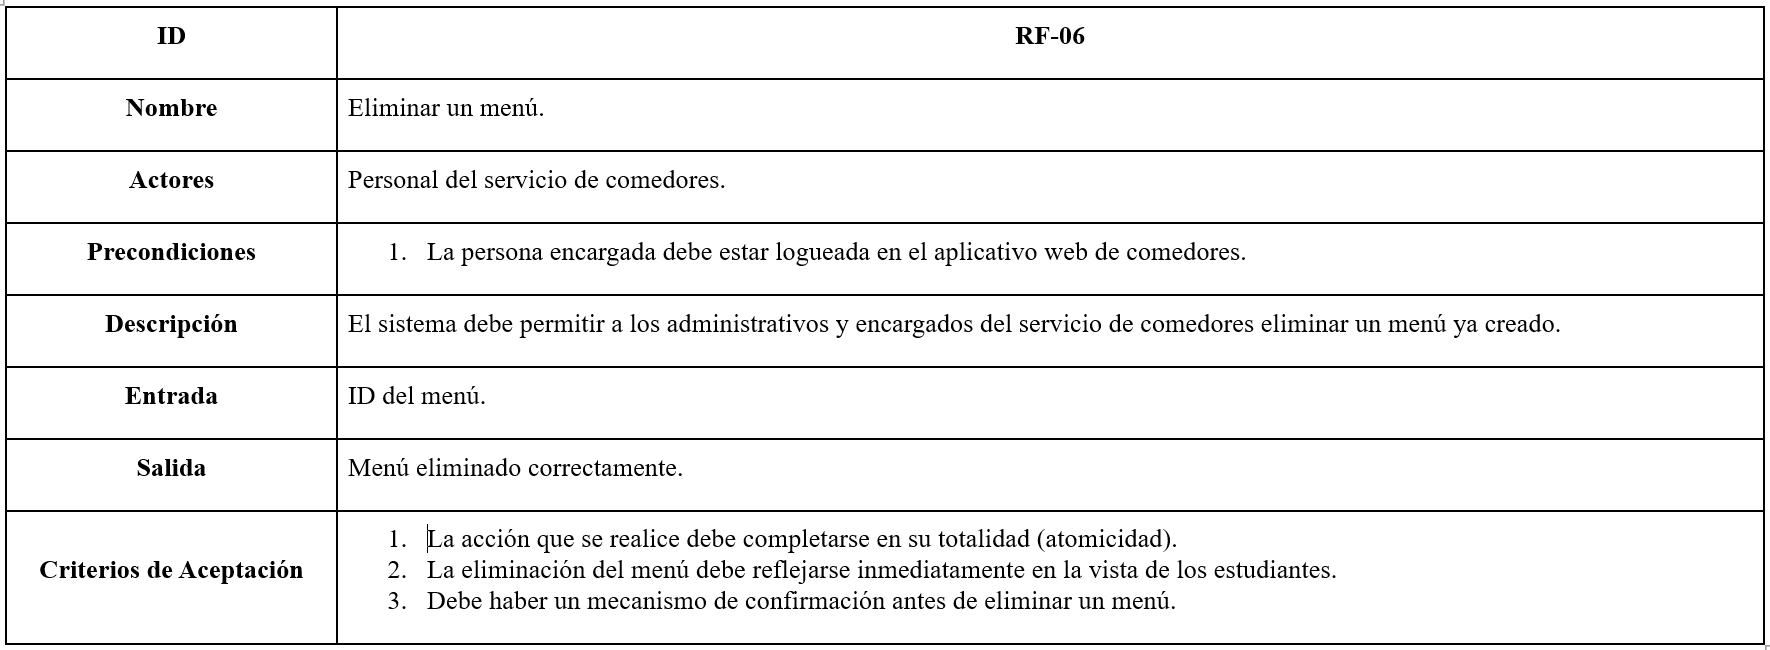
\includegraphics[width=1\linewidth]{Requerimientos Funcionales/6. Requerimiento Funcional.png}
\end{figure}

\begin{figure}[H]
	\caption[]{Séptimo Requerimiento Funcional}
	\label{Séptimo Requerimiento Funcional}
	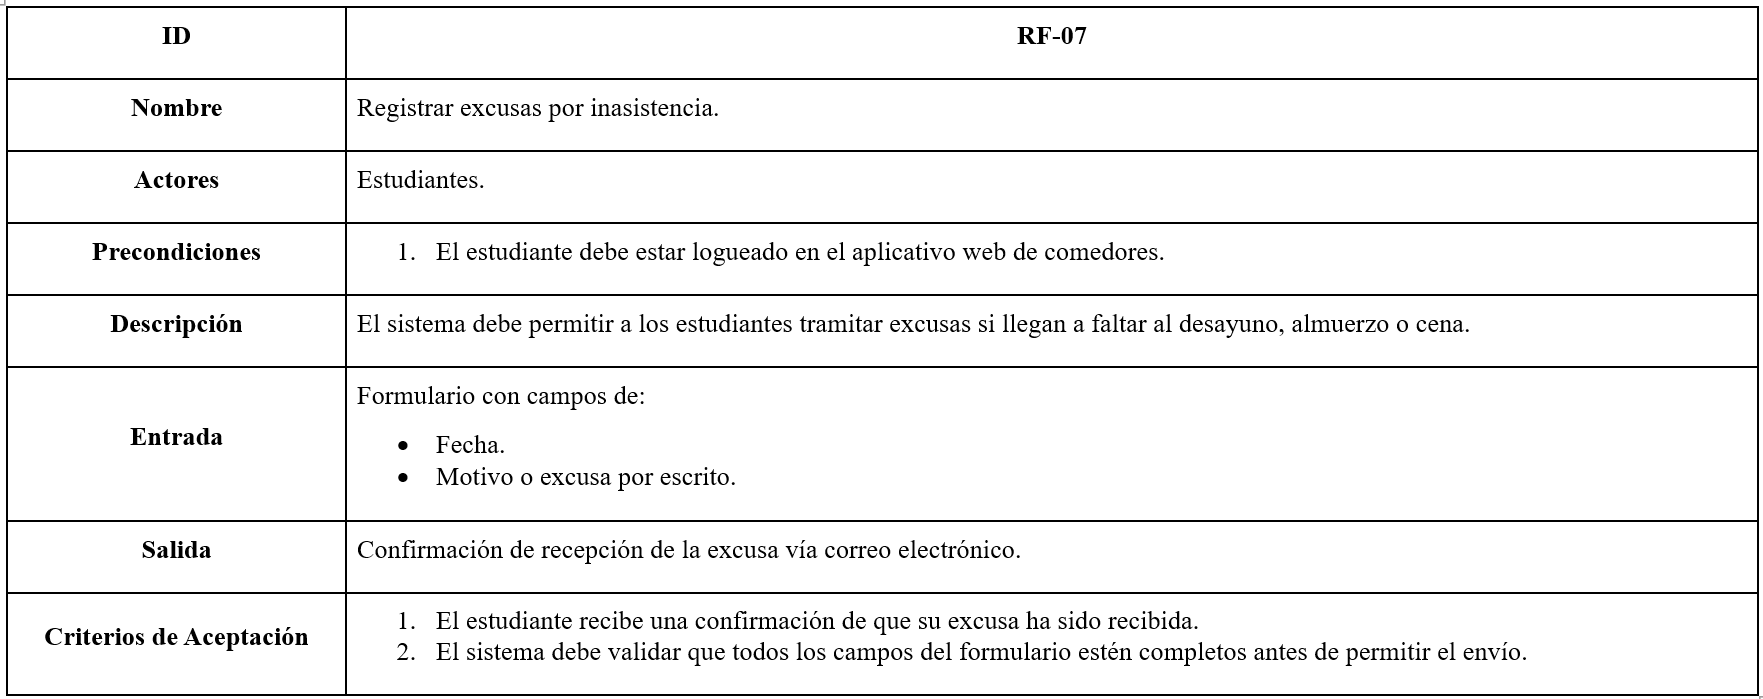
\includegraphics[width=1\linewidth]{Requerimientos Funcionales/7. Requerimiento Funcional.png}
\end{figure}

\newpage
\subsection{Requerimientos No Funcionales}

\begin{figure}[H]
	\caption[]{Primer Requerimiento No Funcional}
	\label{Primer Requerimiento No Funcional}
	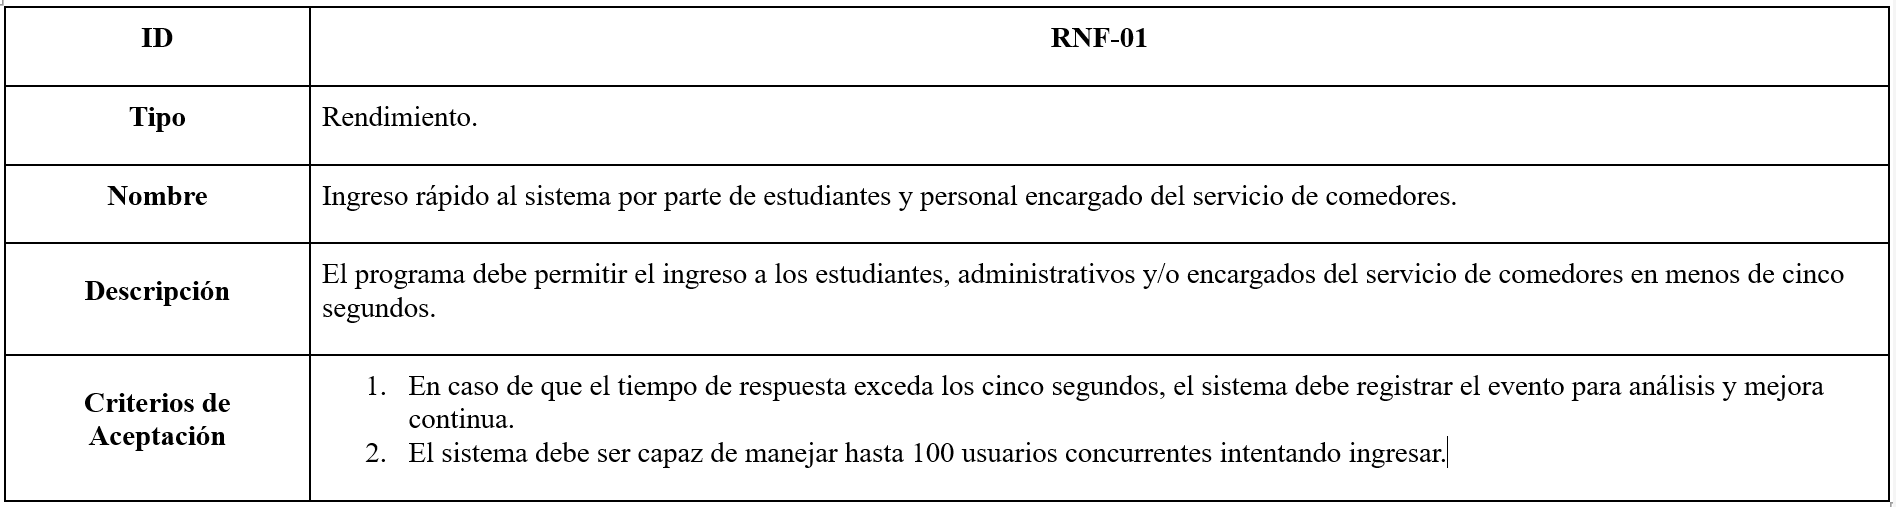
\includegraphics[width=1\linewidth]{Requerimientos No Funcionales/1. Requerimiento No Funcional.png}
\end{figure}

\begin{figure}[H]
	\caption[]{Segundo Requerimiento No Funcional}
	\label{Segundo Requerimiento No Funcional}
	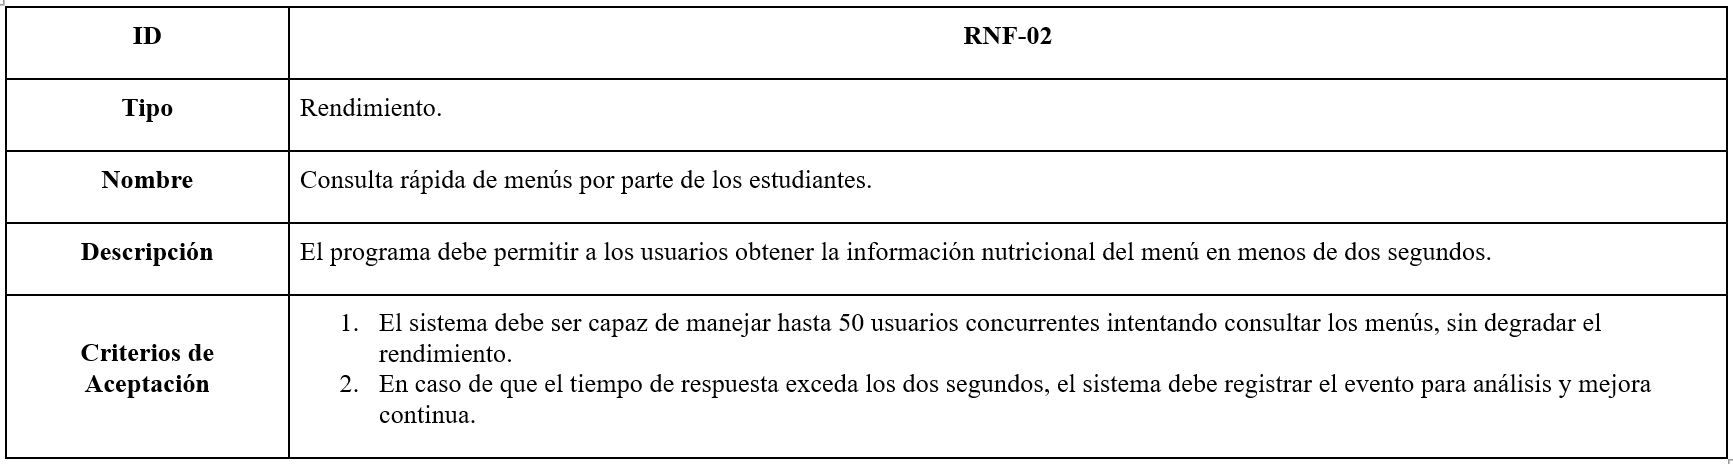
\includegraphics[width=1\linewidth]{Requerimientos No Funcionales/2. Requerimiento No Funcional.png}
\end{figure}

\begin{figure}[H]
	\caption[]{Tercer Requerimiento No Funcional}
	\label{Tercer Requerimiento No Funcional}
	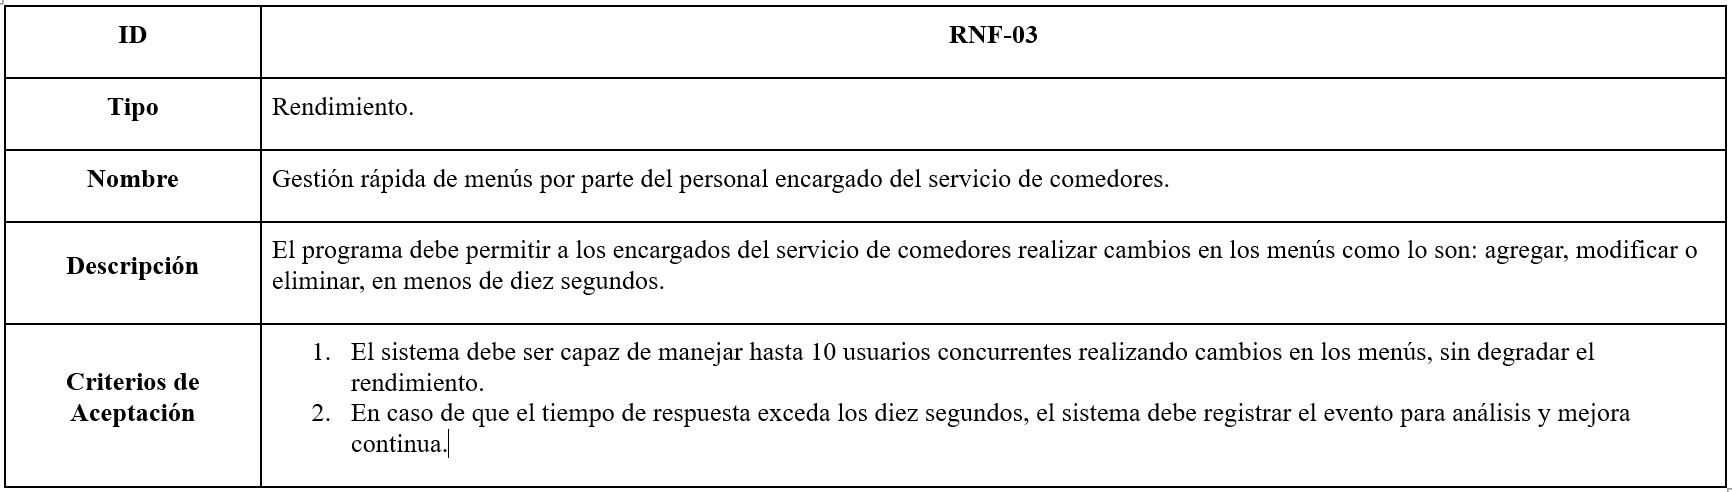
\includegraphics[width=1\linewidth]{Requerimientos No Funcionales/3. Requerimiento No Funcional.png}
\end{figure}

\begin{figure}[H]
	\caption[]{Cuarto Requerimiento No Funcional}
	\label{Cuarto Requerimiento No Funcional}
	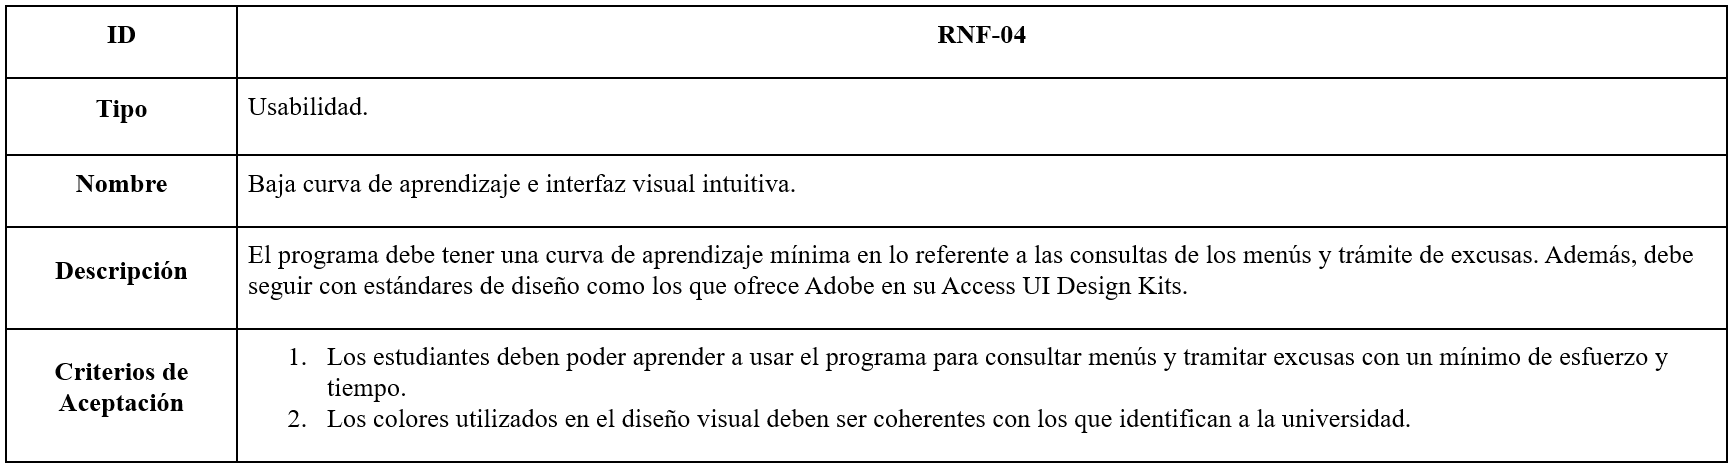
\includegraphics[width=1\linewidth]{Requerimientos No Funcionales/4. Requerimiento No Funcional.png}
	\textit{Nota: Los estándares de diseño de Adobe y los colores usados por la universidad se pueden encontrar en sus respectivos sitios web.}
\end{figure}

\begin{figure}[H]
	\caption[]{Quinto Requerimiento No Funcional}
	\label{Quinto Requerimiento No Funcional}
	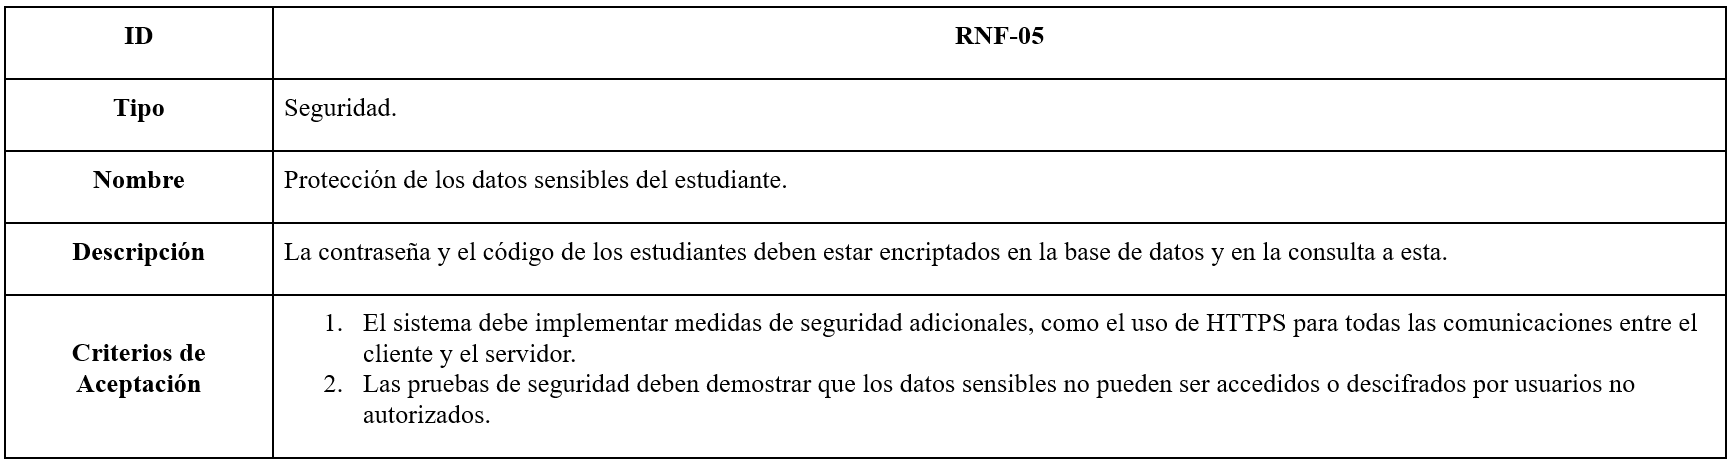
\includegraphics[width=1\linewidth]{Requerimientos No Funcionales/5. Requerimiento No Funcional.png}
\end{figure}

\begin{figure}[H]
	\caption[]{Sexto Requerimiento No Funcional}
	\label{Sexto Requerimiento No Funcional}
	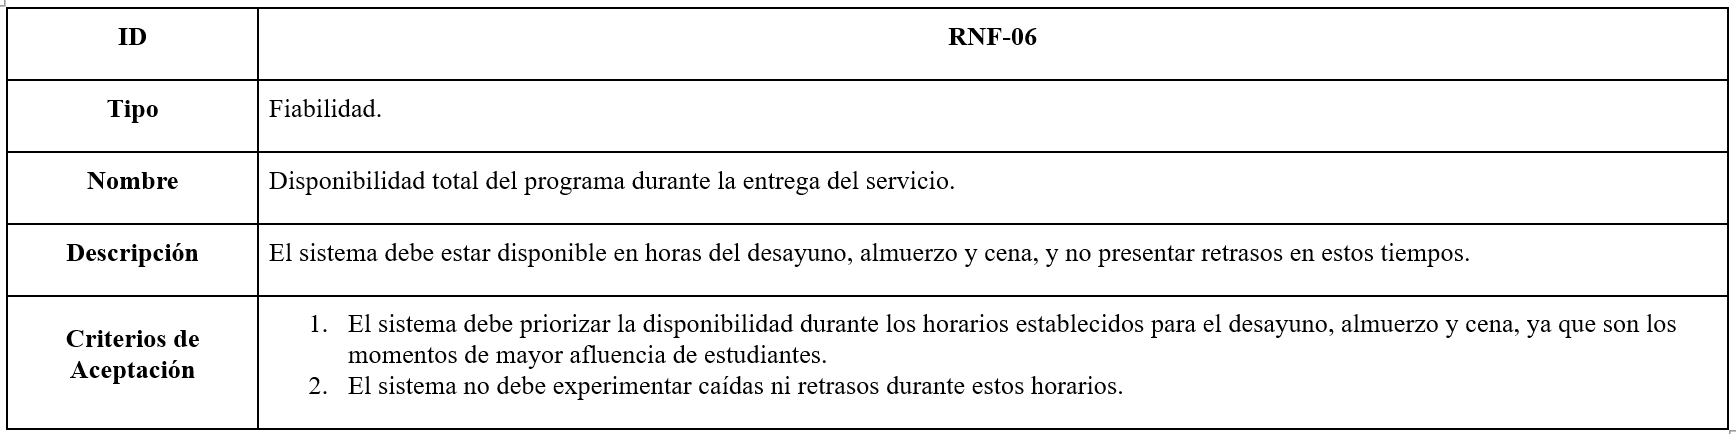
\includegraphics[width=1\linewidth]{Requerimientos No Funcionales/6. Requerimiento No Funcional.png}
\end{figure}

\begin{figure}[H]
	\caption[]{Séptimo Requerimiento No Funcional}
	\label{Séptimo Requerimiento No Funcional}
	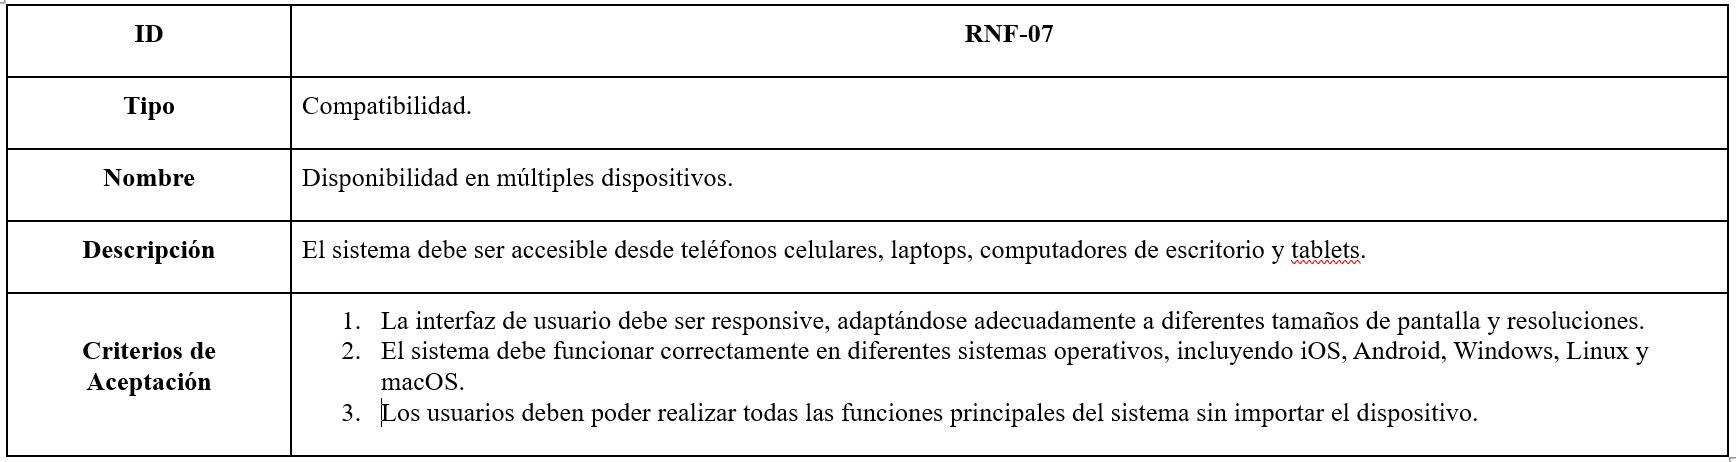
\includegraphics[width=1\linewidth]{Requerimientos No Funcionales/7. Requerimiento No Funcional.png}
\end{figure}

\begin{figure}[H]
	\caption[]{Octavo Requerimiento No Funcional}
	\label{Octavo Requerimiento No Funcional}
	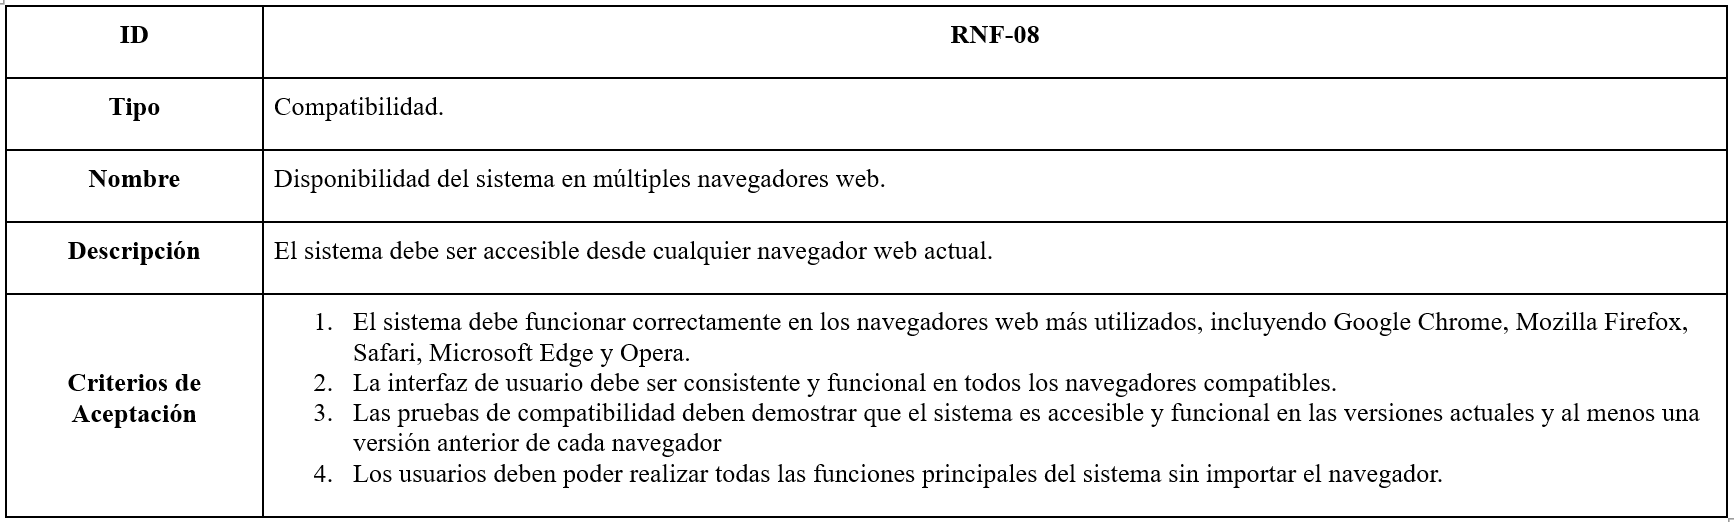
\includegraphics[width=1\linewidth]{Requerimientos No Funcionales/8. Requerimiento No Funcional.png}
\end{figure}

\begin{figure}[H]
	\caption[]{Noveno Requerimiento No Funcional}
	\label{Noveno Requerimiento No Funcional}
	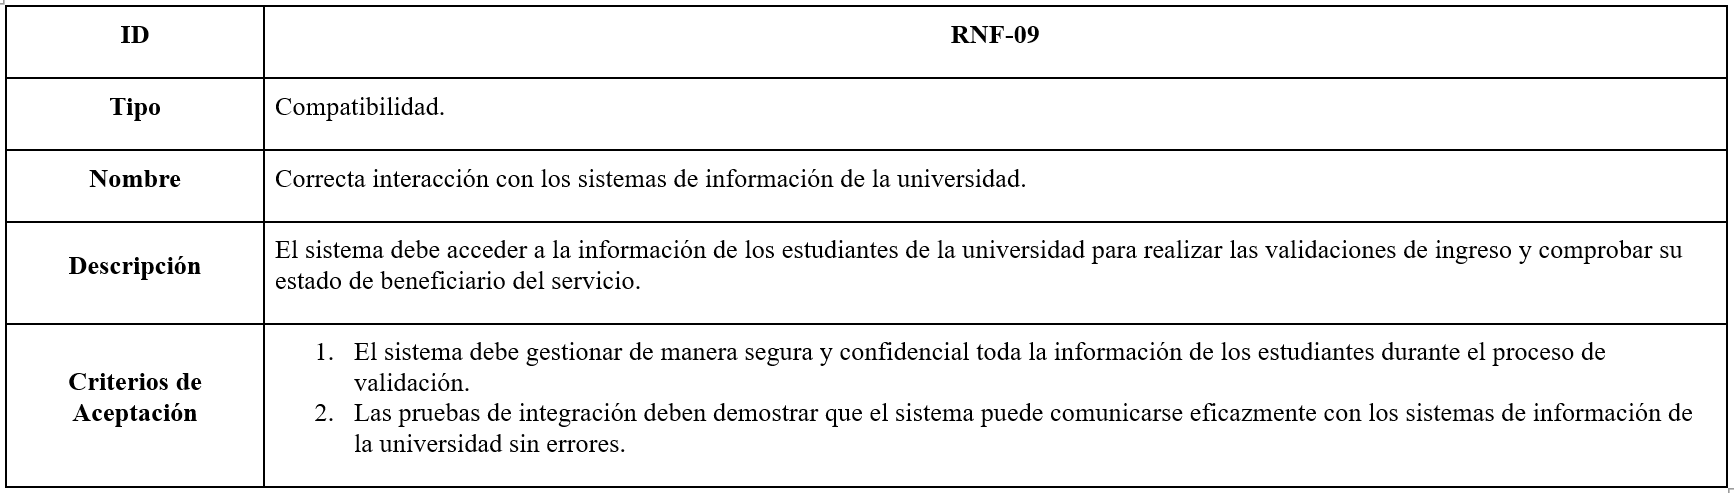
\includegraphics[width=1\linewidth]{Requerimientos No Funcionales/9. Requerimiento No Funcional.png}
\end{figure}

\begin{figure}[H]
	\caption[]{Décimo Requerimiento No Funcional}
	\label{Décimo Requerimiento No Funcional}
	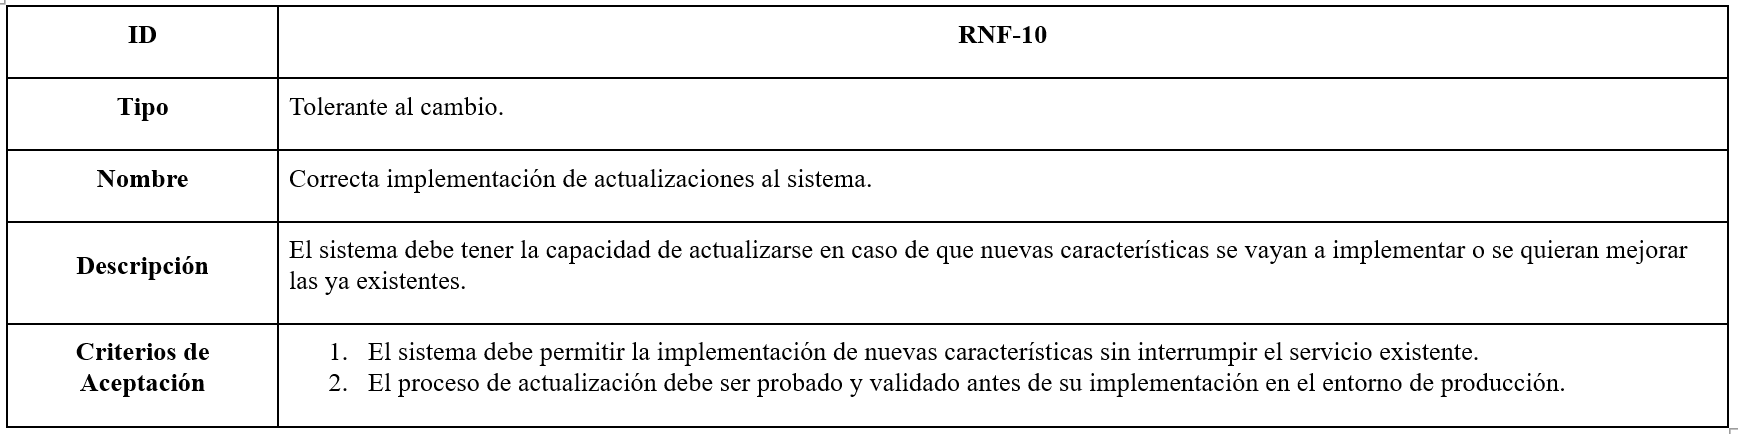
\includegraphics[width=1\linewidth]{Requerimientos No Funcionales/10. Requerimiento No Funcional.png}
\end{figure}

\begin{figure}[H]
	\caption[]{Undécimo Requerimiento No Funcional}
	\label{Undécimo Requerimiento No Funcional}
	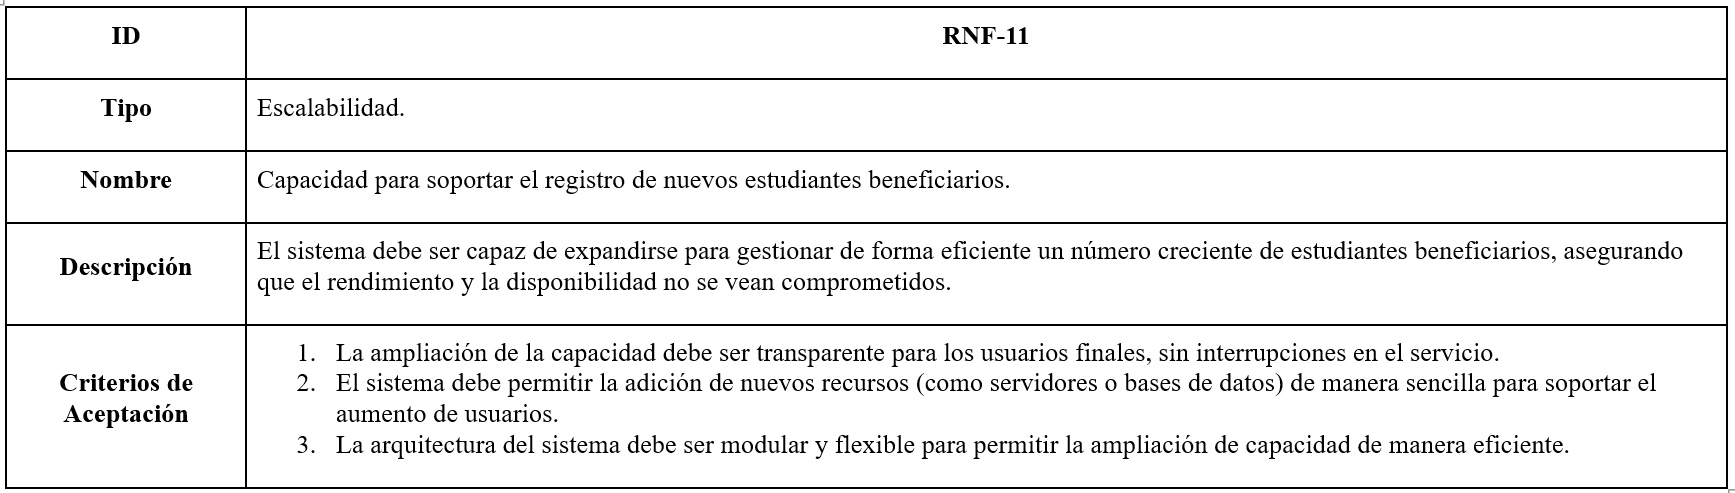
\includegraphics[width=1\linewidth]{Requerimientos No Funcionales/11. Requerimiento No Funcional.png}
\end{figure}

\subsection{Requerimientos de Nivel de Usuario}


\begin{itemize}
	\item \textbf{Historias de Usuario:}
	\begin{itemize}
		\item \textbf{[HU-1] Ingreso al Sistema (Estudiantes):}
		Como estudiante, quiero ingresar al sistema con mi código estudiantil y contraseña para acceder a la información de los menús del día y gestionar mis excusas en caso de ser necesario.
		
		\item \textbf{[HU-2] Consulta de Menús:}
		Como estudiante, quiero consultar los menús diarios para planificar mis comidas y asegurarme de que se ajusten a mis necesidades nutricionales.
		
		\item \textbf{[HU-3] Trámite de Excusas:}
		Como estudiante, quiero tramitar excusas por inasistencia para evitar sanciones innecesarias y mantener un registro claro de mis ausencias.
		
		\item \textbf{[HU-4] Ingreso al Sistema (Personal de Comedores):}
		Como personal del servicio de comedores, quiero ingresar al sistema con mis credenciales para gestionar los menús y la información relacionada con el servicio.
		
		\item \textbf{[HU-5] Creación de Menús:}
		Como personal del servicio de comedores, quiero crear menús junto con su información nutricional para asegurarme de que los estudiantes tengan acceso a datos actualizados.
		
		\item \textbf{[HU-6] Modificación de Menús:}
		Como personal del servicio de comedores, quiero modificar menús ya creados para corregir o agregar información que pueda faltar, garantizando así la precisión y relevancia de los datos.
		
		\item \textbf{[HU-7] Eliminación de Menús:}
		Como personal del servicio de comedores, quiero eliminar menús ya creados para retirar del sistema aquellos que no sean relevantes o hayan sido descontinuados.
		
		\item \textbf{[HU-8] Enviar Notificación al Correo de los Estudiantes:}
		Como personal del servicio de comedores, quiero enviar correos electrónicos desde el aplicativo web a los estudiantes beneficiarios para asegurarme de que estén informados de algún cambio de horarios o determinada información relevante.
	\end{itemize}
\end{itemize}



\subsection{Restricciones}

\begin{itemize}
	\item \textbf{Rendimiento:}
	\begin{itemize}
		\item El sistema debe asegurar tiempos de respuesta inferiores a dos segundos para las operaciones más comunes, como el inicio de sesión y la consulta de menús.
		
		\item Durante los horarios de mayor afluencia (desayuno, almuerzo y cena), el sistema no debe experimentar caídas ni retrasos, garantizando una disponibilidad total.
	\end{itemize}
	
	\newpage
	\item \textbf{Usabilidad:}
	\begin{itemize}
		\item La interfaz del sistema debe ser intuitiva y fácil de usar, permitiendo que los estudiantes y el personal del servicio de comedores realicen todas las funciones principales sin necesidad de capacitación previa y entiendan el funcionamiento en un tiempo no mayor que 30 minutos.
		
		\item La interfaz de usuario debe ser responsive, adaptándose adecuadamente a diferentes tamaños de pantalla y resoluciones, para asegurar que los usuarios puedan acceder al sistema desde diversos dispositivos.
		
		\item Debe incluir mensajes de error claros y comprensibles para los usuarios en caso de que las credenciales ingresadas sean incorrectas.
	\end{itemize}
	
	\item \textbf{Compatibilidad:}
	\begin{itemize}
		\item El sistema debe ser accesible desde los navegadores web más utilizados, incluyendo Google Chrome, Mozilla Firefox, Safari, Microsoft Edge y Opera, garantizando que la interfaz de usuario sea consistente y funcional en todos ellos.
		
		\item El sistema debe funcionar correctamente en diferentes sistemas operativos, incluyendo iOS, Android, Windows, Linux y macOS, asegurando que todos los usuarios puedan acceder sin problemas.
	\end{itemize}
	
	\item \textbf{Seguridad:}
	\begin{itemize}
		\item El sistema debe gestionar de manera segura y confidencial toda la información de los estudiantes durante el proceso de validación.
		
		\item La contraseña y el código de los estudiantes deben estar encriptados en la base de datos y en la consulta a esta.
		
		\item El sistema debe implementar medidas de seguridad adicionales, como el uso de HTTPS para todas las comunicaciones entre el cliente y el servidor.
	\end{itemize}
	
	\item \textbf{Mantenibilidad:}
	\begin{itemize}
		\item El sistema debe permitir la implementación de nuevas características y actualizaciones sin interrumpir el servicio existente, y el proceso de actualización debe ser probado y validado antes de su implementación en el entorno de producción.
		
		\item La documentación del sistema debe estar actualizada para facilitar futuras modificaciones y el trabajo de nuevos desarrolladores.
	\end{itemize}
	
	\item \textbf{Escalabilidad:}
	\begin{itemize}
		\item El sistema debe ser capaz de expandirse para gestionar de forma eficiente un número creciente de estudiantes beneficiarios, asegurando que el rendimiento y la disponibilidad no se vean comprometidos.
		
		\item La arquitectura del sistema debe ser modular y flexible para permitir la ampliación de su capacidad de manera eficiente, facilitando la adición de nuevos recursos como servidores o bases de datos.
	\end{itemize}
	
	\item \textbf{Interoperabilidad:}
	\begin{itemize}
		\item El sistema debe interactuar correctamente con los sistemas de información de la universidad para realizar las validaciones de ingreso y comprobar el estado de beneficiario del servicio, garantizando que no haya errores en la comunicación.
		
		\item Debe permitir la importación y exportación de datos en formatos estándar (CSV, JSON, XML), para facilitar la comunicación con otros sistemas de gestión de la universidad.
	\end{itemize}
\end{itemize}


\newpage
\subsection{Diagramas de Clase}

\subsection{Diagramas de Uso}


\section{Proceso}

\subsection{Reporte SCRUM}

\subsection{Estándares de Ingeniería Usados}

\begin{itemize}
	\item \textbf{UML 2.5.1}
	\begin{itemize}
		\item \textbf{Detalle:} Lenguaje de modelado utilizado para especificar, visualizar, construir y documentar los artefactos de un sistema de software.
		\item \textbf{Uso en el Proyecto:} Durante el diseño y la documentación de la arquitectura del sistema y sus componentes.
	\end{itemize}
	
	\item \textbf{HTTP/2}
	\begin{itemize}
		\item \textbf{Detalle:} Es una versión mejorada del protocolo HTTP que mejora el rendimiento y la eficiencia de las comunicaciones web.
		\item \textbf{Uso en el Proyecto:} Al momento de hacer la comunicación entre el cliente y el servidor web.
	\end{itemize}
	
	\item \textbf{ISO/IEC 27001}
	\begin{itemize}
		\item \textbf{Detalle:} Este estándar especifica los requisitos para establecer, implementar, mantener y mejorar un sistema de gestión de seguridad de la información.
		\item \textbf{Uso en el Proyecto:} Para implementar la protección de la información y gestión de la seguridad de los datos de los estudiantes y el personal encargado del servicio de comedores.
	\end{itemize}
	
	\item \textbf{SCRUM}
	\begin{itemize}
		\item \textbf{Detalle:} Marco de trabajo ágil para la gestión de proyectos y desarrollo de software.
		\item \textbf{Uso en el Proyecto:} Durante la gestión del desarrollo del sistema de comedores universitarios mediante sprints y reuniones iterativas.
	\end{itemize}
	
	\item \textbf{Git}
	\begin{itemize}
		\item \textbf{Detalle:} Sistema de control de versiones distribuido que permite a los desarrolladores gestionar y rastrear cambios en el código fuente.
		\item \textbf{Uso en el Proyecto:} Al momento de gestionar el código fuente, hacer seguimiento de cambios y colaborar entre los desarrolladores.
	\end{itemize}
	
	\item \textbf{Unicode}
	\begin{itemize}
		\item \textbf{Detalle:} Codificación de caracteres que permite representar texto en la mayoría de los sistemas de escritura del mundo.
		\item \textbf{Uso en el Proyecto:} Cuando se hace la representación y manipulación de caracteres en la aplicación web, especialmente en la interfaz gráfica.
	\end{itemize}
	
\end{itemize}

\subsection{Selección de Herramientas}


\section{Solución}

\subsection{Arquitectura de la Solución}

\subsection{Resultado del Desarrollo}


\section{Evaluación}

\subsection{Evaluación Funcional}

\subsection{Evaluación de las Restricciones}

\subsection{Evaluación de la Calidad}


\section{Conclusiones}

\subsection{Trabajo Futuro}

\newpage
\renewcommand\refname{{\textbf{Referencias}}}
\bibliography{mibibliografia}

\end{document}